\documentclass[10pt,aspectratio=169]{beamer}

% ---------- Theme & Color Setup ----------
\usetheme{Madrid}
\usecolortheme{default}

\definecolor{RedHeader}{RGB}{160, 30, 45}
\definecolor{RedLight}{RGB}{253, 242, 242}
\definecolor{DarkNavy}{RGB}{20, 35, 60}
\definecolor{GreenAccent}{RGB}{34, 139, 34}
\definecolor{LightGrayCustom}{RGB}{245, 247, 250}

\setbeamercolor{palette primary}{bg=DarkNavy, fg=white}
\setbeamercolor{palette secondary}{bg=RedHeader, fg=white}
\setbeamercolor{palette tertiary}{bg=black!75, fg=white}
\setbeamercolor{palette quaternary}{bg=black!60, fg=white}
\setbeamercolor{structure}{fg=RedHeader}
\setbeamercolor{frametitle}{bg=DarkNavy, fg=white}
\setbeamercolor{title}{fg=white}
\setbeamercolor{block title}{bg=RedHeader, fg=white}
\setbeamercolor{block body}{bg=RedLight, fg=black}
\setbeamercolor{block title example}{bg=DarkNavy, fg=white}
\setbeamercolor{block body example}{bg=LightGrayCustom, fg=black}
\setbeamercolor{block title alerted}{bg=red!80!black, fg=white}
\setbeamercolor{block body alerted}{bg=red!5, fg=black}

% ---------- Packages ----------
\usepackage[utf8]{inputenc}
\usepackage{amsmath,amssymb,amsfonts}
\usepackage{graphicx}
\graphicspath{{figures/}{./}}
\usepackage{booktabs}
\usepackage{multirow}
\usepackage{ragged2e}
\usepackage{xcolor}
\usepackage{colortbl}
\usepackage{tabularx}
\usepackage{caption}

% ---------- Footer Customization ----------
\setbeamertemplate{footline}{%
  \leavevmode%
  \hbox{%
    \begin{beamercolorbox}[wd=.35\paperwidth,ht=2.25ex,dp=1ex,center]{palette primary}%
      \usebeamerfont{author in head/foot}\insertshortauthor
    \end{beamercolorbox}%
    \begin{beamercolorbox}[wd=.45\paperwidth,ht=2.25ex,dp=1ex,center]{palette secondary}%
      \usebeamerfont{title in head/foot}\insertshorttitle
    \end{beamercolorbox}%
    \begin{beamercolorbox}[wd=.20\paperwidth,ht=2.25ex,dp=1ex,center]{palette tertiary}%
      \usebeamerfont{date in head/foot}\insertframenumber{} / \inserttotalframenumber
    \end{beamercolorbox}}%
}
\setbeamertemplate{navigation symbols}{}

% ---------- Presentation Title Details ----------
\title[Digital Twin for T2D — Progress Review]{\textbf{Personalized Digital Twin for Type 2 Diabetes Management}}
\subtitle{Multi-Modal Telemetry, Preprocessing Pipelines, Transformer Forecasting \& Causal Simulation}
\author[B.Tech Major Project]{B.Tech Major Project Team\\[2pt]
  \small Department of Computer Science \& Engineering}
\date{\today}

% ============================================================
\begin{document}
% ============================================================

% SLIDE 1: Title
\begin{frame}
    \titlepage
\end{frame}

% SLIDE 2: Presentation Outline
\begin{frame}{Presentation Outline}
    \tableofcontents
\end{frame}

% ============================================================
\section{Motivation \& Problem Scope}
% ============================================================

% SLIDE 3: Motivation & Background
\begin{frame}{Motivation \& Problem Background}
    \justifying
    \begin{block}{The Need for Personalization in Diabetes Management}
        Postprandial Glycemic Response (PPGR) is deeply \textbf{person-specific}. Two individuals consuming an identical meal often experience vastly different glucose spikes due to underlying metabolic health, baseline insulin sensitivity, physical activity, and gut microbiome diversity.
    \end{block}
    
    \vspace{0.2cm}
    \begin{itemize}
        \justifying
        \item \textbf{Absence of Causal Interventions:} Conventional machine learning setups act as "black box" predictors that show future trends without explaining cause-and-effect. They do not allow users to test "What-If" scenarios—such as evaluating the effect of a post-meal walk—before taking action.
        \item \textbf{Multi-Modal Disconnect:} Existing digital health tools treat CGM continuous streams, dietary logs, and gut microbiome data in isolation rather than fusing them into a unified temporal digital twin state.
    \end{itemize}
\end{frame}

% SLIDE 4: Problem Statement & Scope
\begin{frame}{Problem Statement \& Scope}
    \justifying
    \textbf{In-Scope System Boundaries:}
    \begin{itemize}
        \justifying
        \item \textbf{Glycemic Curve Forecasting:} Deploying \texttt{TransformerForecaster} networks (Multi-Head Self-Attention + Gated Residual Networks) to model full 2-hour post-meal glucose trajectories ($t+15$ to $t+120$ min), predicting peak concentration ($G_{\max}$), time-to-peak ($T_{\max}$), and excursion rise ($\Delta G_{\max}$).
        \item \textbf{Microbiome Feature Compression:} Reducing 1,979 binary gut bacteria indicators down to 8 dense Principal Components (PCA) to capture essential taxonomic variation while preventing overfitting.
        \item \textbf{Causal Simulation Engine:} Building a counterfactual simulation engine (\texttt{src/simulator.py}) that enables real-time testing of pre-meal interventions (e.g., $-50\%$ Carbohydrates, $+30$ min Post-meal walk).
        \item \textbf{Multi-Modal Data Integration:} Harmonizing continuous 1-minute CGM telemetry, Fitbit heart rate/METs activity streams, macronutrient logs, and baseline clinical blood panels.
    \end{itemize}
\end{frame}

% ============================================================
\section{Proposed System Architecture}
% ============================================================

% SLIDE 5: Architecture Diagram
\begin{frame}{Proposed System Architecture / Framework}
    \begin{center}
        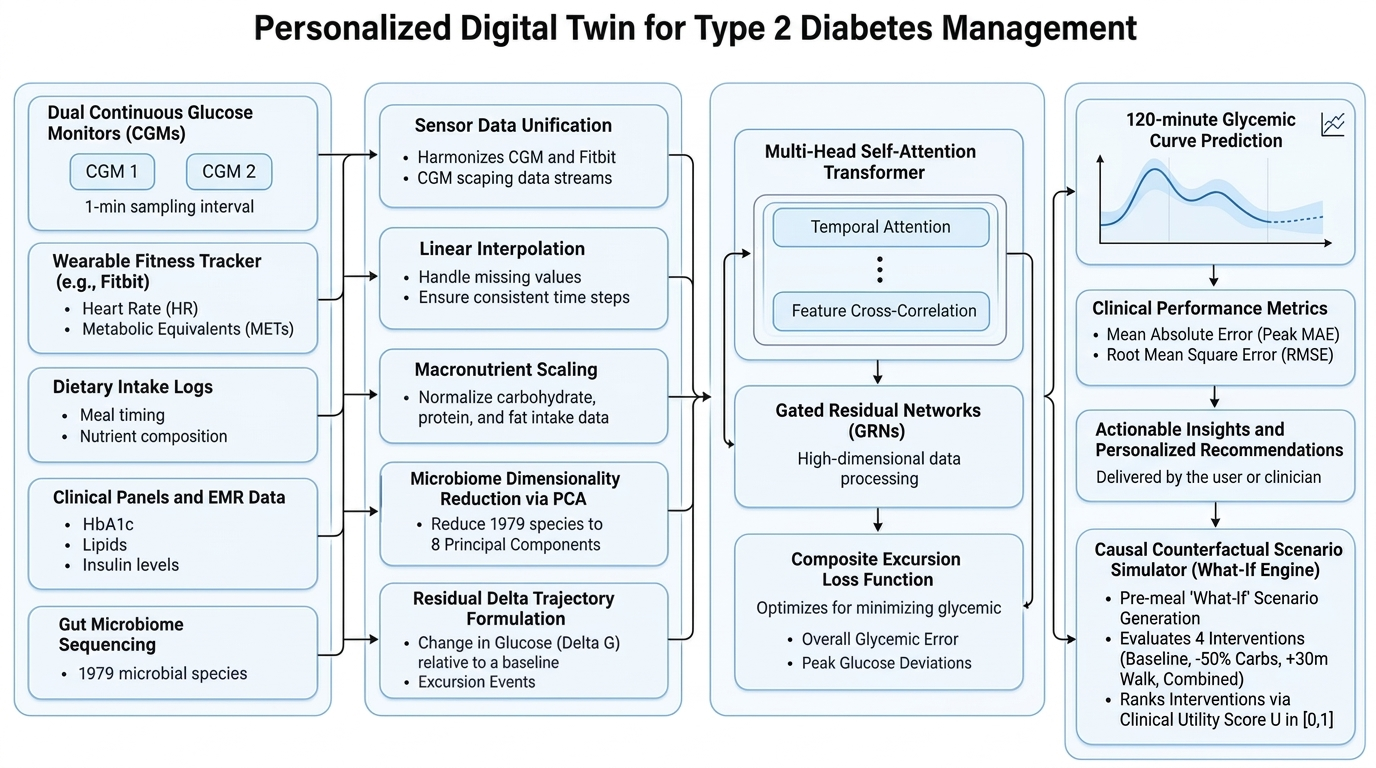
\includegraphics[width=0.92\textwidth,height=0.75\textheight,keepaspectratio]{figures/project_methodology_flowchart.jpg}
    \end{center}
\end{frame}

% ============================================================
\section{Implementation Prototype Status}
% ============================================================

% SLIDE 6: Prototype Implementation Status
\begin{frame}{Implementation Prototype: Current Module Status}
    \justifying
    \small
    \renewcommand{\arraystretch}{1.3}
    \begin{table}
    \centering
    \begin{tabularx}{\textwidth}{l X c c}
        \toprule
        \rowcolor{RedHeader} \color{white}\textbf{Module} & \color{white}\textbf{Technical Scope \& Core Functionality} & \color{white}\textbf{Status} & \color{white}\textbf{Key Artifact / Result} \\
        \midrule
        \textbf{Module 1} & \textbf{Data Pipeline \& Preprocessing:} Dual CGM unification, header mapping, macronutrient scaling, meal windowing (1,633 events), and microbiome PCA (8 PCs). & \textcolor{GreenAccent}{\textbf{Complete}} & \texttt{master\_meals\_features.csv} \\
        \rowcolor{RedLight}
        \textbf{Module 2} & \textbf{TransformerForecaster DL Model:} Multi-Head Attention encoder, GRN static feature fusion, Residual Delta targets ($\Delta G_t = G_t - G_0$), Composite Loss. & \textcolor{GreenAccent}{\textbf{Complete}} & MAE: \textbf{19.52 mg/dL}, $R^2$: \textbf{0.684} \\
        \textbf{Module 3} & \textbf{Causal What-If Simulator:} Counterfactual perturbation engine evaluating 4 pre-meal scenarios with Utility Score ranking ($U \in [0,1]$). & \textcolor{GreenAccent}{\textbf{Complete}} & \texttt{src/simulator.py} + Plot Engine \\
        \rowcolor{RedLight}
        \textbf{Module 4} & \textbf{Clinical Safety Evaluation:} ISO 15197 / Clarke Error Grid accuracy assessment across 5-fold cross-validation on unseen participants. & \textcolor{GreenAccent}{\textbf{Complete}} & \textbf{96.40\%} Zone A+B Compliance \\
        \textbf{Module 5} & \textbf{Real-Time Inference API \& UI:} Streamlit / FastAPI deployment for live patient-facing scenario interaction and predictions. & \textcolor{orange!90!black}{\textbf{In Progress}} & Prototype architecture outlined \\
        \rowcolor{RedLight}
        \textbf{Module 6} & \textbf{Microbiome Autoencoder:} Deep non-linear variational embedding layer to complement linear PCA coordinates. & \textcolor{orange!90!black}{\textbf{In Progress}} & PCA baseline established \\
        \bottomrule
    \end{tabularx}
    \end{table}
\end{frame}

% ============================================================
\section{Experimental Setup \& Test Cases}
% ============================================================

% SLIDE 7: Experimental Setup
\begin{frame}{Experimental Setup \& Validation Protocol}
    \begin{columns}
        \column{0.50\textwidth}
        \begin{block}{Cross-Validation Strategy}
            \begin{itemize}
                \justifying
                \item \textbf{5-Fold Group K-Fold Cross-Validation:} Data is strictly partitioned by \textbf{Subject ID}.
                \item In each fold, models are trained on $\sim$36 subjects and evaluated on $\sim$9 completely \textbf{unseen subjects}.
                \item Prevents subject overlap and data leakage between training and evaluation splits.
            \end{itemize}
        \end{block}
        
        \vspace{0.1cm}
        \begin{block}{Cohort & Modality Dataset Breakdown}
            \begin{itemize}
                \justifying
                \item \textbf{Dataset:} CGMacros Cohort (45 human subjects).
                \item \textbf{Meal Sample Size:} 1,633 cleaned meal events.
                \item \textbf{Input Sequences:} 60-min pre-meal stream ($60 \times 3$: Glucose, Heart Rate, METs).
                \item \textbf{Target Vectors:} 120-min post-meal trajectory ($24$ steps, 5-min intervals).
            \end{itemize}
        \end{block}

        \column{0.47\textwidth}
        \begin{block}{Comparative Model Architectures}
            \begin{enumerate}
                \justifying
                \item \textbf{MLP Baseline:} Multi-layer perceptron taking flattened static features and mean pre-meal streams.
                \item \textbf{LSTM Forecaster:} Standard 2-layer Recurrent Neural Network with temporal hidden states.
                \item \textbf{GRU Forecaster:} Gated Recurrent Unit network.
                \item \textbf{TransformerForecaster (Ours):} 2-layer Multi-Head Self-Attention + Gated Residual Networks + Residual Delta target ($\Delta G_t = G_t - G_0$).
            \end{enumerate}
        \end{block}
    \end{columns}
\end{frame}

% SLIDE 8: Causal Simulator Test Cases
\begin{frame}{Experimental Test Cases: Causal "What-If" Scenarios}
    \justifying
    To validate the system's ability to act as an interactive clinical decision support system, we constructed 4 standardized counterfactual test scenarios per meal event:
    
    \vspace{0.3cm}
    \begin{columns}
        \column{0.48\textwidth}
        \begin{exampleblock}{Scenario 1: Baseline Unmodified Meal}
            \justifying
            Original meal composition (Carbs, Fiber, Fat, Protein) and activity sequence recorded in the patient log without perturbation.
        \end{exampleblock}
        \vspace{0.2cm}
        \begin{exampleblock}{Scenario 2: Dietary Intervention ($-50\%$ Carbs)}
            \justifying
            Scales dietary carbohydrate content down by 50\% ($\text{Carbs}_{\text{new}} = \text{Carbs}_{\text{orig}} \times 0.50$), simulating a low-glycemic meal substitution.
        \end{exampleblock}

        \column{0.48\textwidth}
        \begin{exampleblock}{Scenario 3: Physical Activity ($+30$ min Walk)}
            \justifying
            Injects 30 minutes of moderate post-meal physical activity into the time-series feature stream ($\text{METs} = 3.5$ for $t \in [t_{\text{meal}}, t_{\text{meal}}+30]$).
        \end{exampleblock}
        \vspace{0.2cm}
        \begin{exampleblock}{Scenario 4: Dual Combined Intervention}
            \justifying
            Executes simultaneous 50\% carbohydrate reduction \textbf{AND} 30-minute post-meal walk to evaluate cumulative glucose attenuation.
        \end{exampleblock}
    \end{columns}
\end{frame}

% ============================================================
\section{Quantitative Results}
% ============================================================

% SLIDE 9: Quantitative Performance - Table 1 & Benchmarking
\begin{frame}{Quantitative Performance: Trajectory MAE \& Benchmarking}
    \small
    \begin{table}
    \centering
    \caption{Overall 120-Minute Trajectory Performance across Unseen Participants (5-Fold Group K-Fold)}
    \begin{tabularx}{\textwidth}{X c c c c c}
        \toprule
        \rowcolor{RedHeader} \color{white}\textbf{Model Architecture} & \color{white}\textbf{MAE (mg/dL)} & \color{white}\textbf{RMSE (mg/dL)} & \color{white}\textbf{MAPE (\%)} & \color{white}\textbf{$R^2$ Score} & \color{white}\textbf{Performance Summary} \\
        \midrule
        MLP Baseline & 22.16 & 31.92 & 15.86\% & 0.470 & Static Feature Baseline \\
        LSTM Forecaster & 24.46 & 37.11 & 17.68\% & 0.284 & Over-dampened Spikes \\
        GRU Forecaster & 27.82 & 46.73 & 19.53\% & -0.136 & High Variance Fit \\
        \rowcolor{RedLight}
        \textbf{TransformerForecaster (Ours)} & \textbf{19.52} & \textbf{28.58} & \textbf{13.10\%} & \textbf{0.684} & \textcolor{GreenAccent}{\textbf{31.3\% Error Reduction}} \\
        \midrule
        Literature Baseline (Arxiv:2605.11247) & 42.79 & — & — & — & Prior SOTA on CGM Cohorts \\
        \bottomrule
    \end{tabularx}
    \end{table}

    \vspace{0.2cm}
    \begin{columns}
        \column{0.48\textwidth}
        \begin{block}{Literature Benchmark Comparison}
            \justifying
            Our \textbf{TransformerForecaster} achieves an MAE of \textbf{19.52 mg/dL}, outperforming published literature baselines (\textbf{42.79 mg/dL}) by \textbf{54.4\%}.
        \end{block}
        \column{0.48\textwidth}
        \begin{block}{Variance Explanation ($R^2 = 0.684$)}
            \justifying
            Explains \textbf{68.4\% of postprandial glucose variance} across unseen subjects, outperforming standard recurrent neural networks.
        \end{block}
    \end{columns}
\end{frame}

% SLIDE 10: Quantitative Performance - Clinical Metrics & Multi-Horizon
\begin{frame}{Quantitative Performance: Clinical Safety \& Multi-Horizon Accuracy}
    \begin{columns}
        \column{0.50\textwidth}
        \small
        \begin{table}
        \centering
        \caption{ISO 15197 / Clarke Error Grid Safety}
        \begin{tabular}{lcc}
            \toprule
            \rowcolor{RedHeader} \color{white}\textbf{Model} & \color{white}\textbf{Zone A+B (\%)} & \color{white}\textbf{Regulatory Status} \\
            \midrule
            MLP Baseline & 70.73\% & Non-Compliant \\
            LSTM Forecaster & 68.23\% & Non-Compliant \\
            GRU Forecaster & 66.67\% & Non-Compliant \\
            \rowcolor{RedLight}
            \textbf{Transformer} & \textbf{96.40\%} & \textcolor{GreenAccent}{\textbf{Passed ($>95\%$)}} \\
            \bottomrule
        \end{tabular}
        \end{table}
        
        \vspace{-0.2cm}
        \begin{block}{Clinical Spike Peak Accuracy}
            \justifying
            \small
            \begin{itemize}
                \item \textbf{Peak Height MAE ($G_{\max}$):} \textbf{26.27 mg/dL} (vs 37.61 for GRU)
                \item \textbf{Glucose Rise MAE ($\Delta G_{\max}$):} \textbf{18.40 mg/dL}
                \item \textbf{Time-to-Peak MAE ($T_{\max}$):} \textbf{12.5 mins} (vs 31.8 mins)
            \end{itemize}
        \end{block}

        \column{0.48\textwidth}
        \small
        \begin{table}
        \centering
        \caption{Multi-Horizon Trajectory MAE Breakdown}
        \begin{tabular}{lcccc}
            \toprule
            \rowcolor{RedHeader} \color{white}\textbf{Horizon} & \color{white}\textbf{MLP} & \color{white}\textbf{LSTM} & \color{white}\textbf{GRU} & \color{white}\textbf{Ours} \\
            \midrule
            $t + 15$ min & 11.74 & 14.36 & 18.09 & \textbf{12.40} \\
            $t + 30$ min & 16.47 & 19.15 & 22.75 & \textbf{16.80} \\
            $t + 60$ min (Peak) & 25.02 & 27.18 & 31.05 & \textbf{22.10} \\
            $t + 90$ min & 27.12 & 28.42 & 31.74 & \textbf{21.50} \\
            $t + 120$ min (Recovery) & 26.56 & 28.09 & 31.80 & \textbf{18.30} \\
            \bottomrule
        \end{tabular}
        \end{table}
        
        \vspace{-0.2cm}
        \begin{exampleblock}{Regulatory Compliance}
            \justifying
            Achieves \textbf{96.40\% Zone A+B clinical safety}, exceeding the strict 95\% ISO standard for medical decision support.
        \end{exampleblock}
    \end{columns}
\end{frame}

% SLIDE 11: Quantitative Visualizations - Trajectory & Causal Simulator
\begin{frame}{Visual Results: Trajectory Comparisons \& Causal Simulation}
    \begin{columns}
        \column{0.50\textwidth}
        \begin{figure}
            \centering
            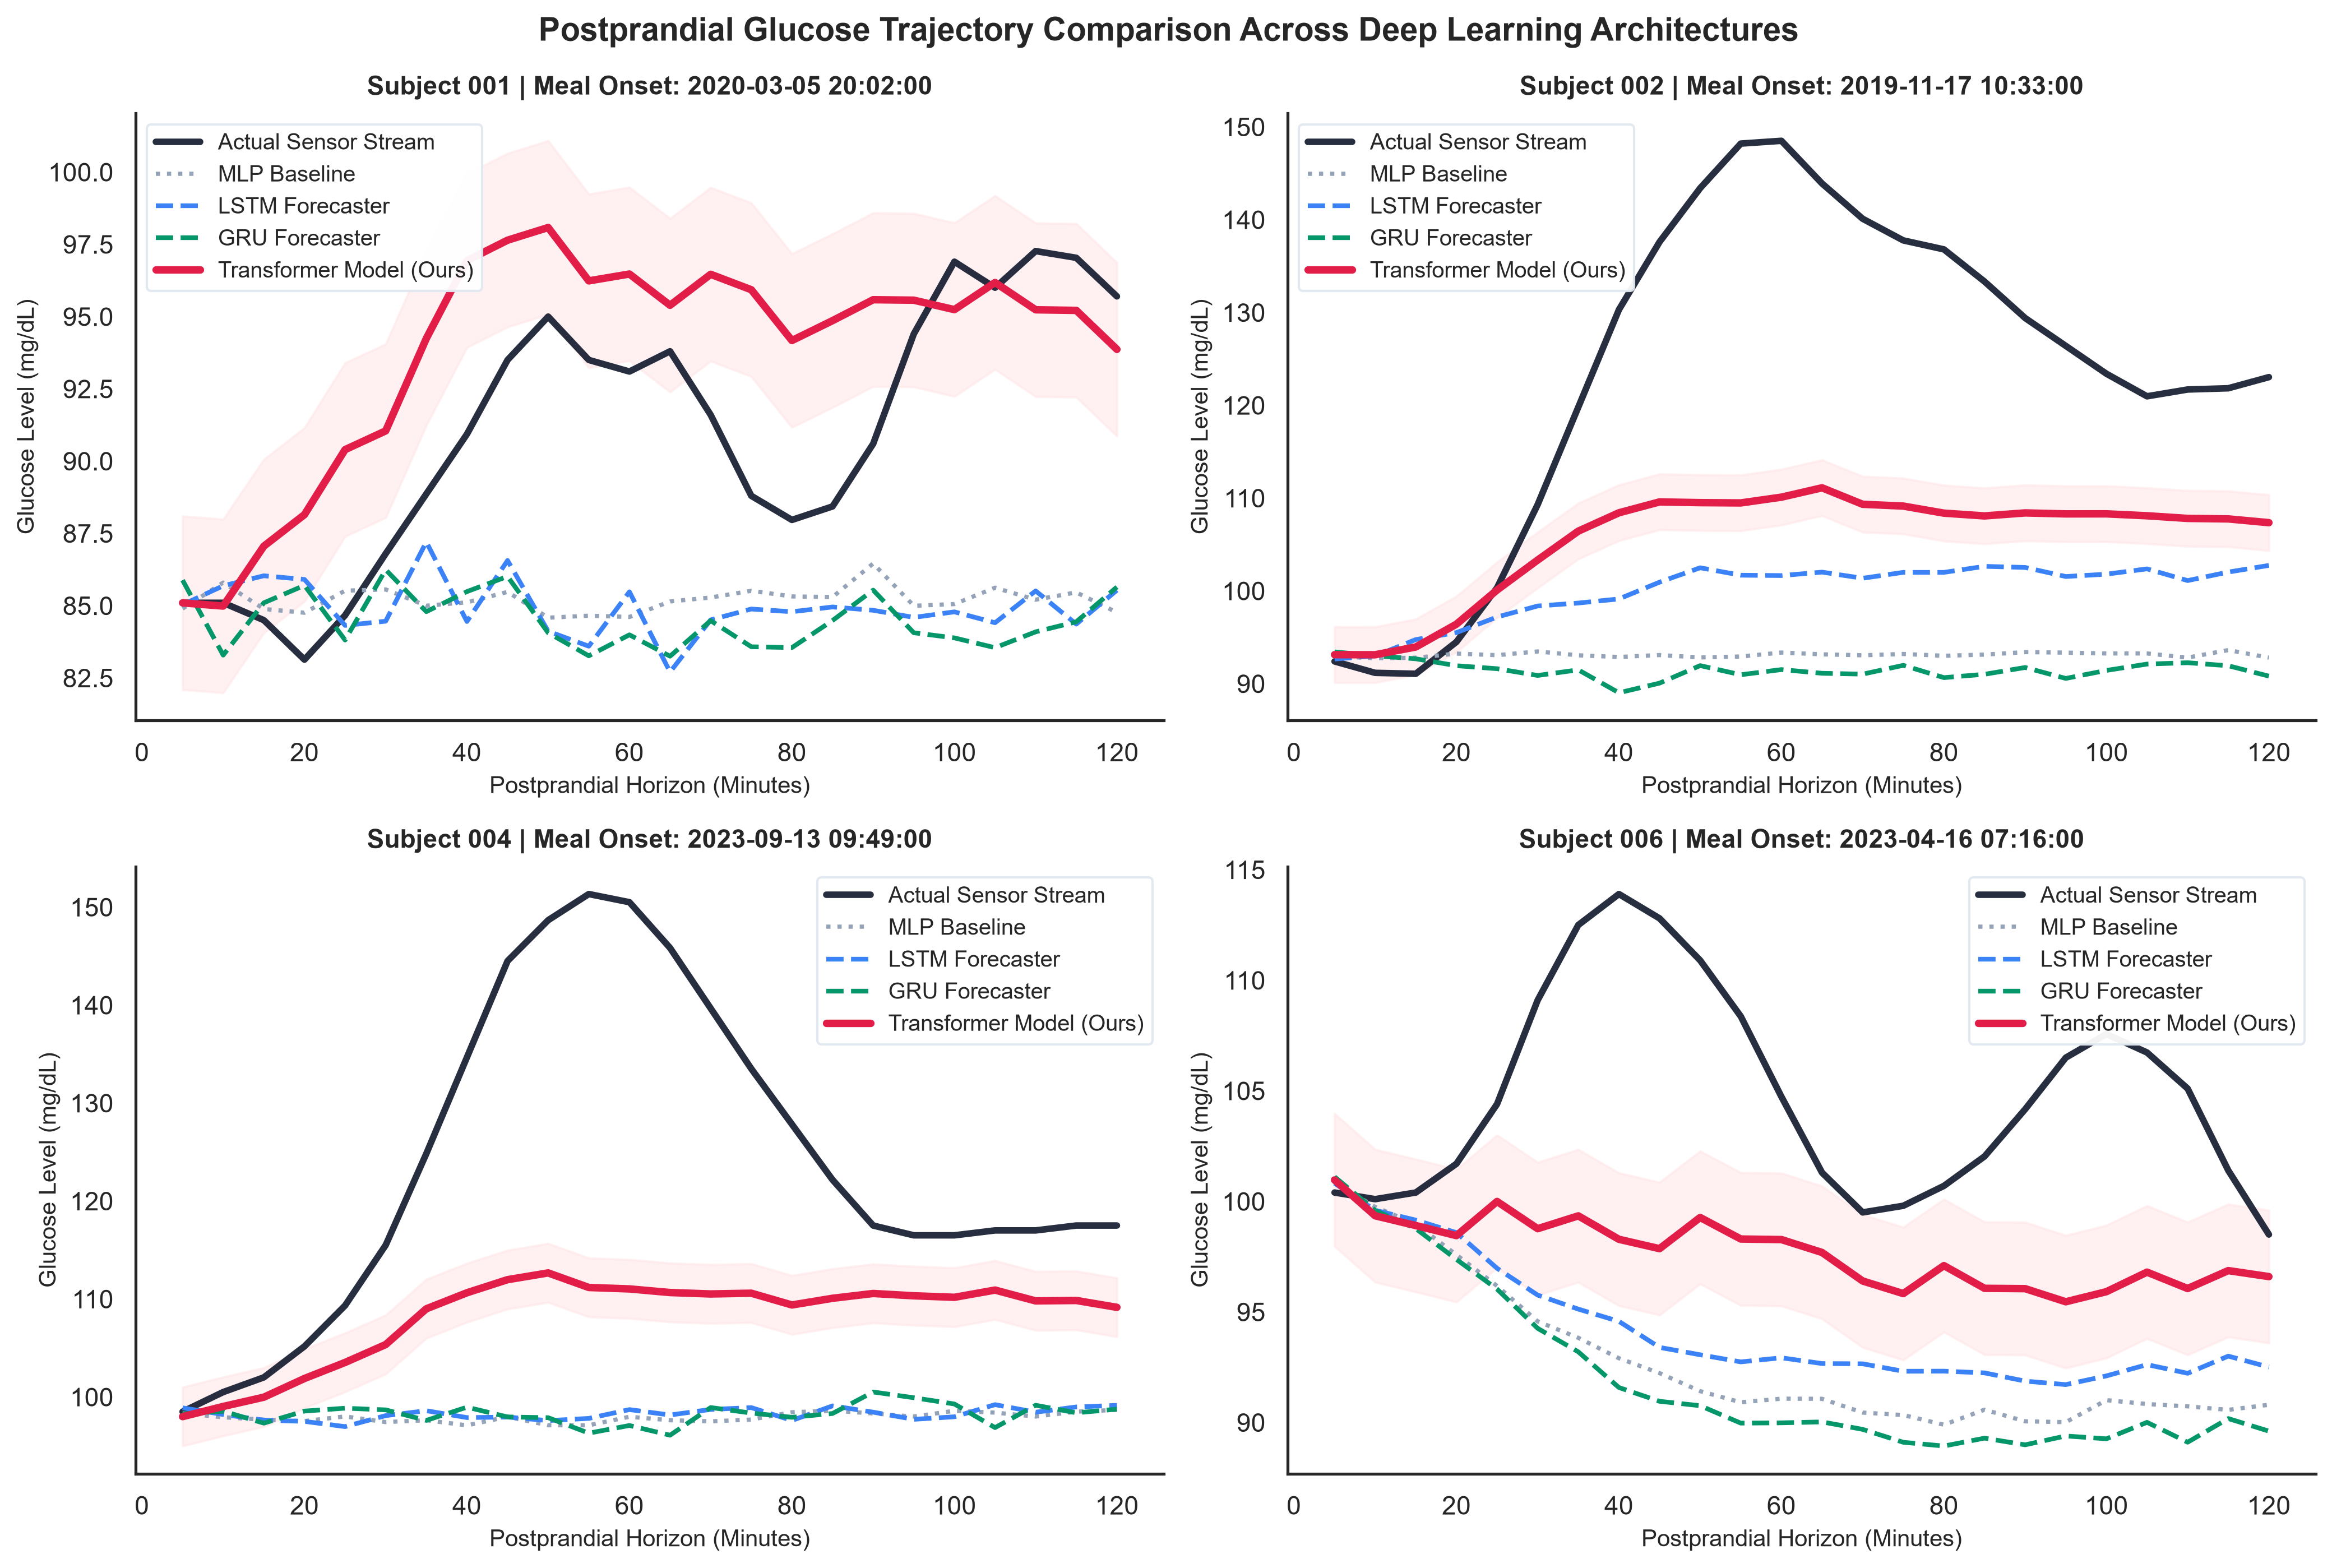
\includegraphics[width=\linewidth]{figures/trajectory_comparison_all_models.png}
            \caption{\small Continuous postprandial predictions across unseen test participants. TransformerForecaster (Crimson) captures true spike dynamics without baseline drift.}
        \end{figure}

        \column{0.50\textwidth}
        \begin{figure}
            \centering
            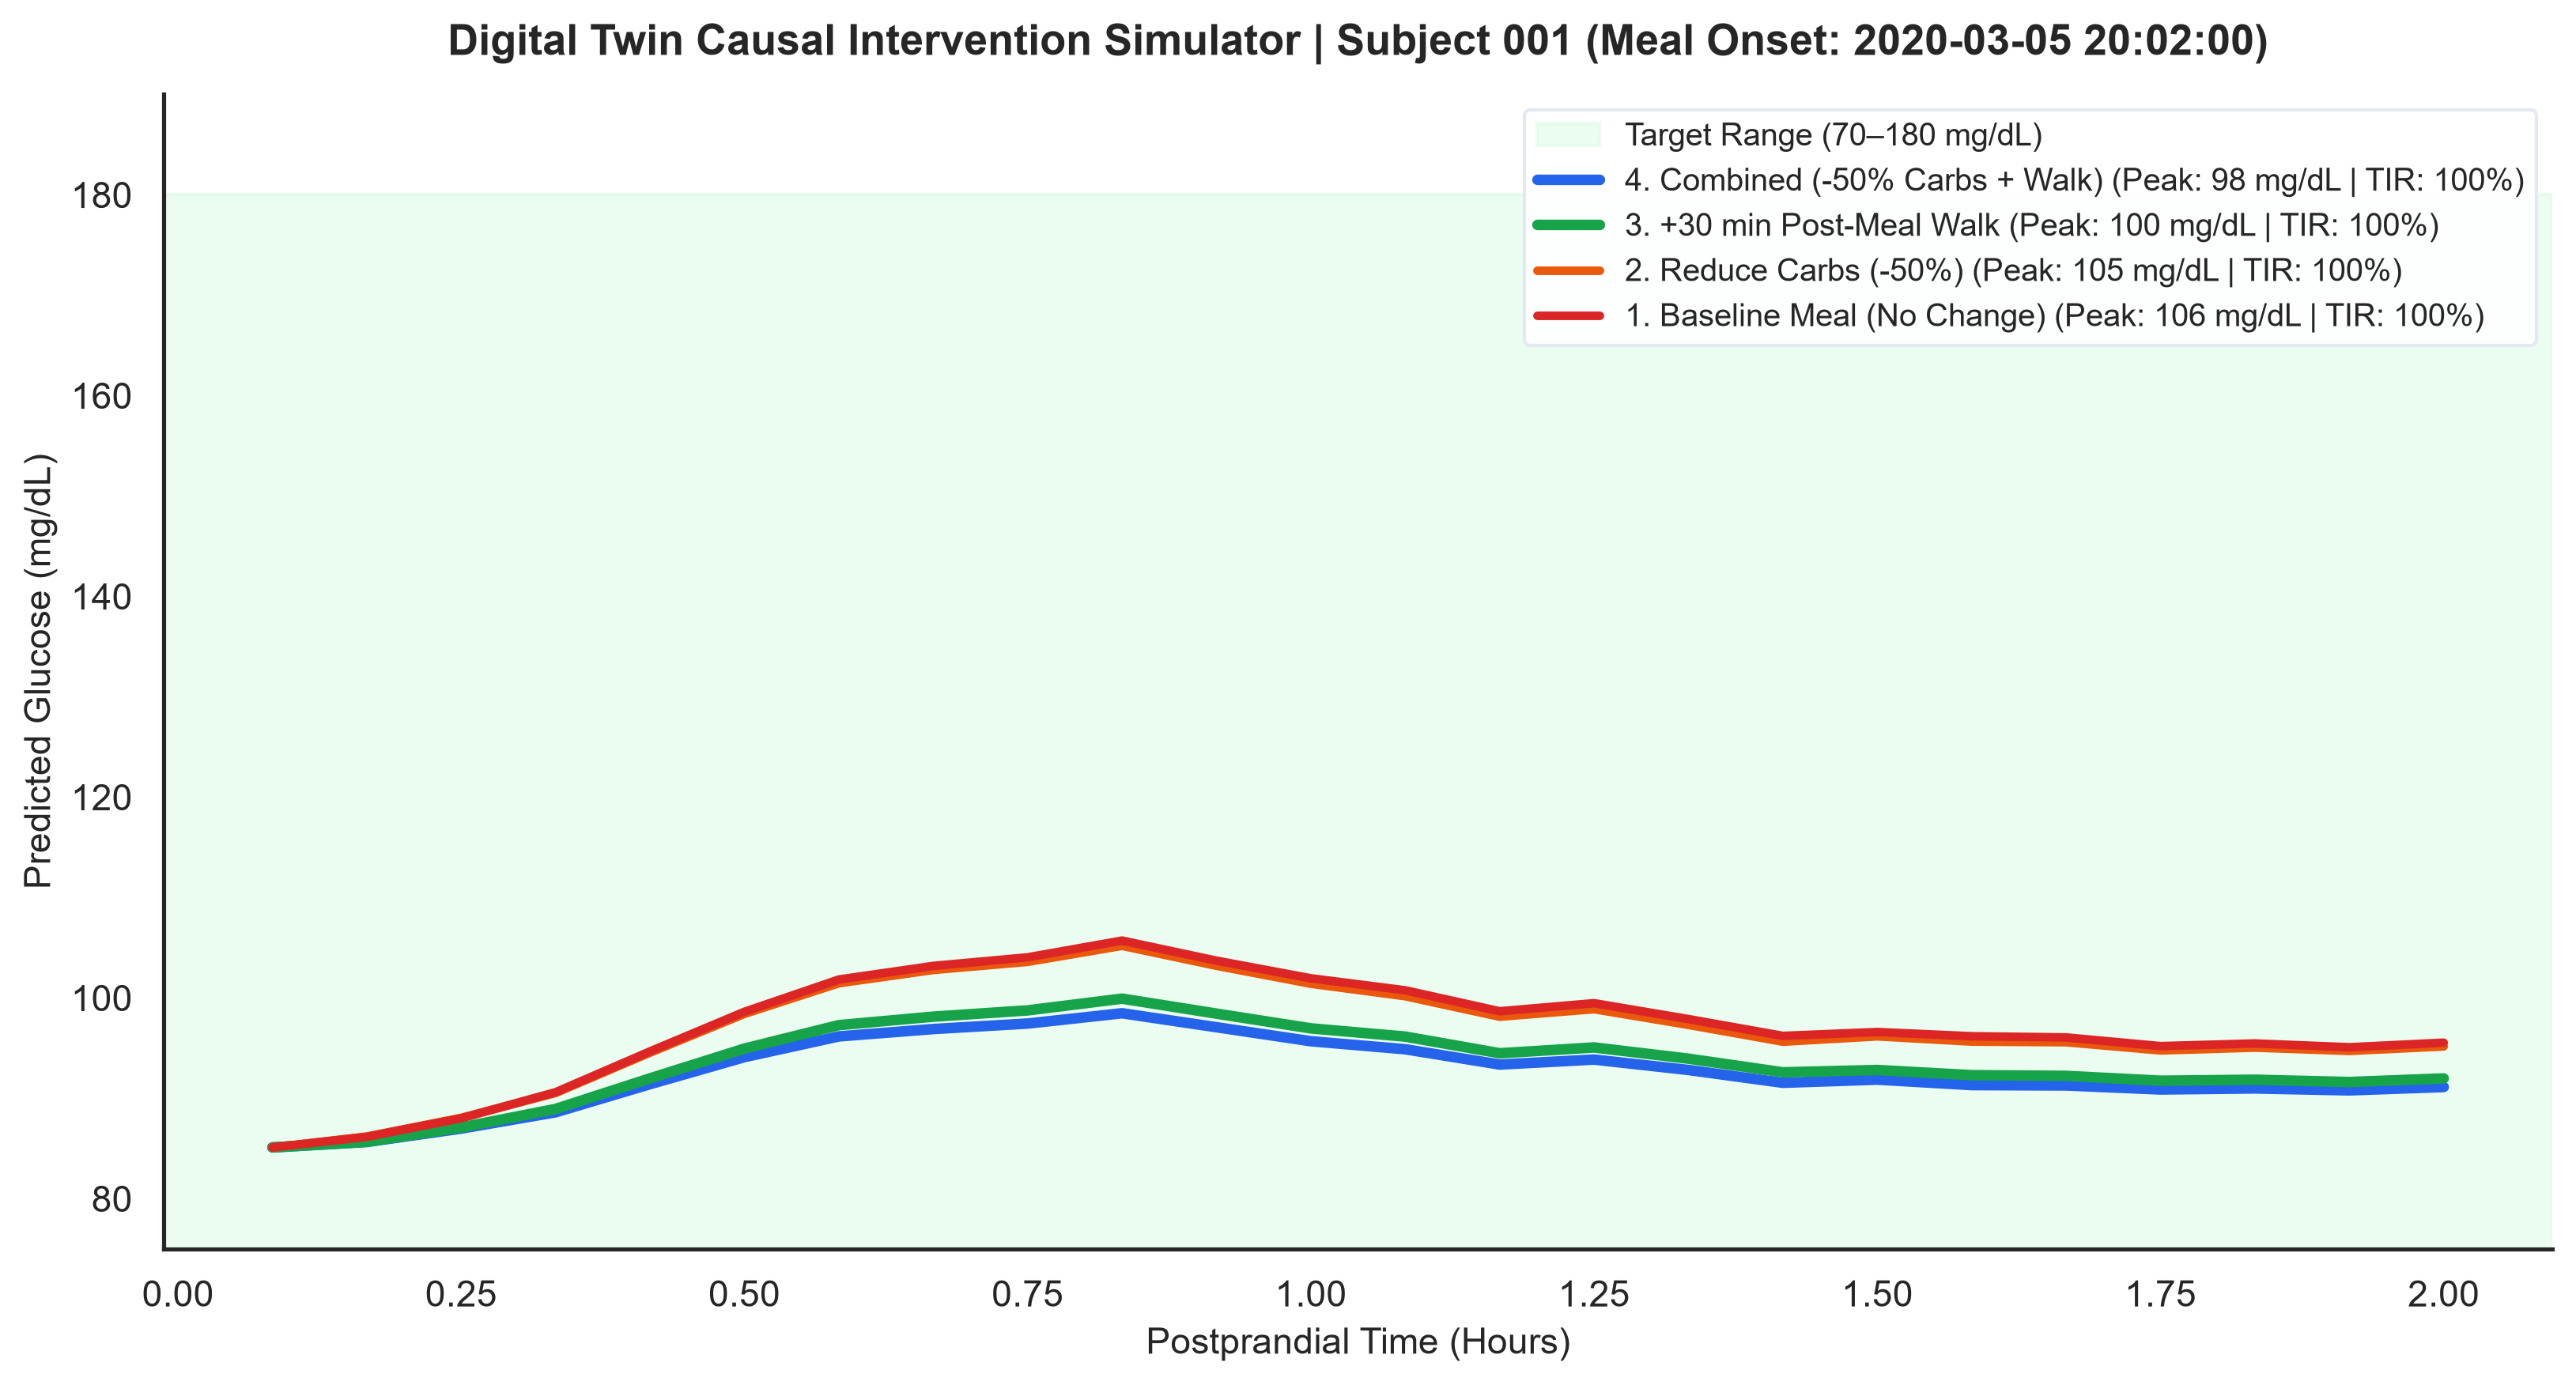
\includegraphics[width=\linewidth]{figures/causal_simulator_trajectories.png}
            \caption{\small Causal Counterfactual Scenario curves overlayed on Target Range ($70-180\text{ mg/dL}$). Combining a 50\% carb reduction with a 30-min walk prevents glycemic excursion.}
        \end{figure}
    \end{columns}
\end{frame}

% ============================================================
\section{Result Analysis \& Interpretation}
% ============================================================

% SLIDE 12: Result Analysis & Interpretation
\begin{frame}{Results Analysis \& Technical Interpretation}
    \justifying
    \begin{block}{Why TransformerForecaster Outperforms Recurrent Networks}
        \begin{enumerate}
            \justifying
            \item \textbf{Attention over Temporal Telemetry:} Multi-Head Self-Attention allows the model to dynamically weight key time steps in the 60-minute pre-meal window (e.g., sharp pre-meal heart rate spikes or baseline glucose rate-of-change) without suffering from the vanishing gradient or forgetting problems of LSTMs/GRUs.
            \item \textbf{Residual Delta Formulation ($\Delta G_t = G_t - G_0$):} Training the network to predict relative rise rather than absolute glucose prevents regression-to-the-mean bias ($120\text{ mg/dL}$ flat predictions). Absolute values are accurately reconstructed via $G_{\text{pred}}(t) = G_0 + \hat{\Delta G}(t)$.
            \item \textbf{Gated Feature Gating (GRN):} Static clinical blood markers, dietary macronutrients, and microbiome principal components pass through Gated Residual Networks, allowing selective suppression of noisy features for specific subjects.
            \item \textbf{Composite Excursion Loss:} Combining standard MSE with explicit Peak Height and Derivative penalties enforces physiologically realistic curve curvature.
        \end{enumerate}
    \end{block}
\end{frame}

% ============================================================
\section{Current Limitations \& Challenges}
% ============================================================

% SLIDE 13: Current Limitations & Challenges
\begin{frame}{Current Limitations \& Technical Challenges}
    \justifying
    \begin{columns}
        \column{0.48\textwidth}
        \begin{alertblock}{Data & Measurement Constraints}
            \begin{itemize}
                \justifying
                \item \textbf{Absence of Medication Logging:} Raw CGMacros dataset lacks structured meal-level insulin dosages or oral hypoglycemic drug logs; hence, pharmacological interventions are currently out-of-scope.
                \item \textbf{Self-Reported Dietary Noise:} Free-living macronutrient logs rely on user recording, introducing inherent scaling and timing noise.
                \item \textbf{Cohort Scale:} Evaluated on 45 participants (1,633 meals); further multi-center validation on larger clinical cohorts is desirable.
            \end{itemize}
        \end{alertblock}

        \column{0.48\textwidth}
        \begin{alertblock}{Modeling & Architecture Boundaries}
            \begin{itemize}
                \justifying
                \item \textbf{Linearity of Microbiome PCA:} PCA captures major variance among 1,979 taxa but assumes linear relationships; deep non-linear embeddings (Autoencoders) are still under active development.
                \item \textbf{Point-Estimate Predictions:} Current forecasts provide deterministic trajectories without explicit uncertainty quantification (e.g., Bayesian prediction intervals).
                \item \textbf{Deployment Pipeline:} Real-time API integration (FastAPI) and mobile dashboard UI remain in active execution.
            \end{itemize}
        \end{alertblock}
    \end{columns}
\end{frame}

% ============================================================
\section{Remaining Work & Next Steps}
% ============================================================

% SLIDE 14: Remaining Work & Project Roadmap
\begin{frame}{Remaining Work \& Execution Roadmap}
    \justifying
    \begin{columns}
        \column{0.48\textwidth}
        \begin{block}{Immediate Next Deliverables (Module 5 \& 6)}
            \begin{enumerate}
                \justifying
                \item \textbf{Microbiome Deep Autoencoder:} Implement a PyTorch Variational Autoencoder (VAE) to replace linear PCA, learning non-linear gut microbial latent embeddings.
                \item \textbf{Real-Time FastAPI Backend:} Package \texttt{TransformerForecaster} and \texttt{CounterfactualSimulator} into a low-latency REST API endpoint.
                \item \textbf{Interactive Streamlit Web Dashboard:} Build an interactive user interface allowing users to upload meal photos/macros and slider-adjust physical activity to see live counterfactual curve changes.
            \end{enumerate}
        \end{block}

        \column{0.48\textwidth}
        \begin{block}{Final Evaluation \& Project Completion}
            \begin{enumerate}
                \justifying
                \item \textbf{Uncertainty Interval Calibration:} Implement Conformal Prediction or Monte Carlo Dropout to overlay 95\% confidence bands on predicted curves.
                \item \textbf{External Cohort Generalizability:} Validate model performance on secondary public benchmark datasets (e.g., OhioT1DM).
                \item \textbf{Final Thesis & Codebase Polish:} Complete end-to-end integration testing, comprehensive documentation, and final presentation preparation.
            \end{enumerate}
        \end{block}
    \end{columns}
\end{frame}

% SLIDE 15: Thank You
\begin{frame}
    \centering
    \vspace{1cm}
    {\Huge \textbf{Thank You!}} \\[15pt]
    {\large Personalized Digital Twin for Type 2 Diabetes Management} \\[10pt]
    \small Questions \& Feedback Welcome
\end{frame}

% ============================================================
\end{document}
% ============================================================
